\chapter{Background on Convolutional Neural Networks}\label{ch:cnn}

\begin{figure}[t!]
\centering
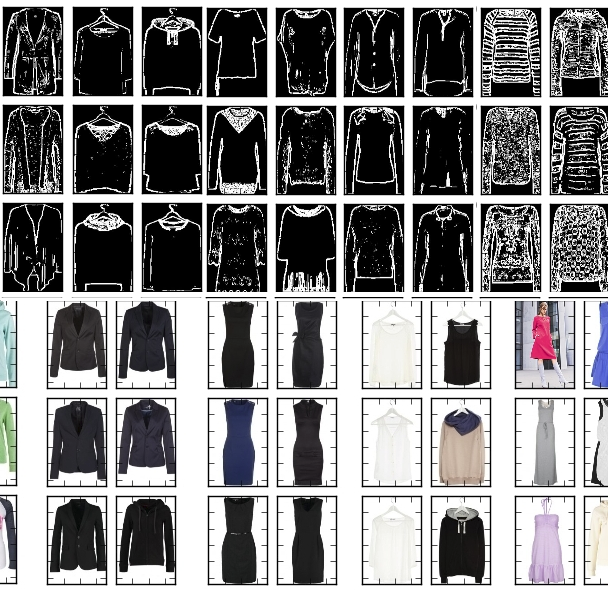
\includegraphics[width=.48\linewidth]{figs/convolution.png}
\caption{Applying a feature mask over a set of fashion items to extract necessary information for auto-encoding. Unnecessary information for example color or brand emblems are not saved. This feature map is an edge detection mask that leaves only shape information which helps to distinguish between different types of clothes.} 
\label{fig:convolution}
\end{figure}


When used for image recognition, convolutional neural networks consist of multiple layers of feature maps that extract different information on small portions of the input image. How many layers and feature maps is tunable to increase the matching process. The output of these collections are then tiled so that they overlap to gain a better representation of the original image and allow for translation. To truly understand CNNs, a breakdown of what convolution means with regards to imaging is necessary. Convolution of an image is using a map of some sort to extract features from the input image by matrix multiplication. The map is multiplied to a small image patch and this is then saved. This is done until the whole image is processed and what is left is a feature map that has the important features extracted. An example of convolution for the process of object identification is shown in figure \ref{fig:convolution}. In this figure you can see how an edge detection feature map is used to save only necessary information for recognizing different types of clothes. You can also see by having multiple feature maps you can get more detail or less detail from an image which can then simplify or complicate the object recognition task. Being able to distinguish between a shirt or a leg garment is as much information you want, having a feature map that extracts outline edge or shape information would be all that you need. But if instead you wanted to distinguish between a formal cocktail dress or a summer dress, more information would need to be saved equating to many more feature maps for one image. Rather than trying to come up with a scheme of feature maps to run over the image by hand, CNNs do this automatically. CNNs take input parameters, for example number of layers, number of units per layers, number of connections per unit, and uses these to create the feature maps. The layers build upon each-other, for example if we were creating a CNN for facial recognition the convolutional layers will start learning feature combinations off of the previous layers. The simple edges, gradients, and corners of the first layers become things like eyes, noses, and hairs in later layers. This process is visualized in figure \ref{fig:featuremaps} 

\begin{figure}[h!]
\centering
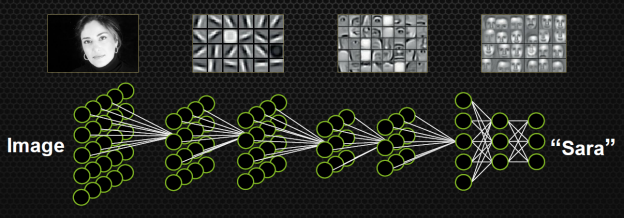
\includegraphics[width=.9\linewidth]{figs/facialDetection.png}
\caption{Pictorial Representation of Convolutional Neural Networks as well as a visual representation on CNN's complexity of layer feature extraction}
\label{fig:featuremaps}
\end{figure}

\section{AlexNet}
\section{GoogleNet}
